\documentclass{article}

\usepackage[left=2cm, right=2cm, top=2cm, bottom=2cm]{geometry}
\usepackage{fancyhdr}
\usepackage{float}
\usepackage{graphicx}
\graphicspath{{./images}}
\usepackage{hyperref}

\renewcommand{\figurename}{Ábra}

\pagestyle{fancy}
\lhead{Webes alkalmazások fejlesztése}
\rhead{2023/2024 tavaszi félév}
\cfoot{\thepage}

\begin{document}
	\section*{Beadandó feladat dokumentáció}
	\subsection*{Feladat}
	Készítsünk egy mozi üzemeltető rendszert, mely két alkalmazásból áll. Az első egy webes felület, melyen keresztül a nézők megtekinthetik a moziműsort, valamint rendelhetnek jegyeket.
	\begin{itemize}
		\item A főoldalon megjelenik a napi program, azaz mely filmeket mikor vetítik a moziban, valamint kiemelve az öt legfrissebb (legutoljára felvitt) film plakátja.
		\item A filmet kiválasztva megjelenik annak részletes leírása (rendező, főszereplők, hossz, szinopszis), plakátja, továbbá az összes előadás időpontja.
		\item Az időpontot kiválasztva lehetőség nyílik helyfoglalásra az adott előadásra. Ekkor a felhasználónak meg kell adnia a lefoglalandó ülések helyzetét (sor, illetve oszlop) egy, a mozitermet sematikusan ábrázoló grafikus felületen. Egyszerre legfeljebb 6 jegy foglalható, és természetesen csak a szabad helyek foglalhatóak (amelyek nem foglaltak, vagy eladottak). A felhasználónak ezen felül meg kell adnia teljes nevét, valamint telefonszámát, ezzel véglegesíti a foglalást.
	\end{itemize}
	A második egy asztali grafikus felület, melyet az alkalmazottak használnak a mozipénztárakban az előadások meghirdetésére, illetve jegyek kiadására.
	\begin{itemize}
		\item Az alkalmazott bejelentkezhet (felhasználónév és jelszó megadásával) a programba, illetve kijelentkezhet.
		\item Új film felvitelekor ki kell tölteni a film adatait (cím, rendező, főszereplők, hossz, szinopszis), valamint feltölthetünk egy képet plakátként.
		\item Új előadás meghirdetéséhez a felhasználónak ki kell választania a termet, valamint a filmet, és az időpont megadásával hirdetheti meg az előadást. A meghirdetéskor ügyelni kell arra, hogy az előadás ne ütközzön más előadásokkal az adott teremben (figyelembe véve a kezdés időpontját, illetve a film hosszát), illetve két előadás között legalább 15 percnek kell eltelnie a takarítás végett.
		\item A jegyvásárláshoz ki kell választani a filmet és az előadást. Ezt követően listázódnak a helyek (sor, oszlop, státusz). A szabad, illetve foglalt helyek eladhatóak, illetve a foglalt helyeket kiválasztva meg lehet tekinteni a foglaló adatait (név, telefonszám).
	\end{itemize}
	\subsection*{Elemzés}
	\begin{itemize}
		\item A feladat megoldása négy komponens, egy adatbázis (illetve annak adatátviteli osztályai), egy webes felhasználói felület, egy webszolgáltatás és az azt használó asztali grafikus felület. Az adatbázis az Entity Framework, a webes felhasználói felület (illetve webszolgáltatás) ASP.NET CORE és Razor, illetve az asztali grafikus felület WPF keretrendszerek segítségével készülnek.
		\item A webes felhasználói felület három weblapon fog megjelenni:
		\begin{enumerate}
			\item weblap a főoldal, melyen megjelenik a napi program, azaz mely filmeket mikor vetítik a moziban, valamint kiemelve az öt legfrissebb (legutoljára felvitt) film plakátja.
			\item weblap, mely az 1. weblapon való film választása után megjeleníti annak részletes leírását (rendező, főszereplők, hossz, szinopszis), plakátját, továbbá az összes aznapi előadás időpontját.
			\item weblap, melyen a 2. weblapon való időpont kiválasztása után lehetőség nyílik helyfoglalásra az adott előadásra. Ekkor a felhasználónak meg kell adnia a lefoglalandó ülések helyzetét (sor, illetve oszlop) egy, a mozitermet sematikusan ábrázoló grafikus felületen. Egyszerre legfeljebb 6 jegy foglalható, és természetesen csak a szabad helyek foglalhatóak (amelyek nem foglaltak, vagy eladottak). A felhasználónak ezen felül meg kell adnia teljes nevét, valamint telefonszámát, ezzel véglegesíti a foglalást.
		\end{enumerate}
		\item Az asztali grafikus felület két ablakban, melyből az egyik három lapon (fülön) fog megjelenni:
		\begin{enumerate}
			\item ablak az alkalmazás elindításakor először megjelenített, ahol az alkalmazott bejelentkezhet a programba.
			\item ablak, mely tartalmazza az egyes funkciókhoz kötött oldalakat
			\begin{enumerate}
				\item[1.] oldala, ahol listázhatóak a filmek és azokhoz adható új, illetve a meglevőket lehet frissíteni és törölni.
				\item[2.] oldala, ahol listázhatóak az előadások és azokhoz adható új, illetve a meglevőket lehet frissíteni és törölni.
				\item[3.] oldala, ahol listázhatóak a másodikon választott előadás ülései, melyek közül a szabad és foglalt ülésekre lehet jegyet kiadni.
			\end{enumerate}
		\end{enumerate}
	\end{itemize}
	\subsection*{Felhasználói esetek}
	\begin{figure}[H]
		\centering
		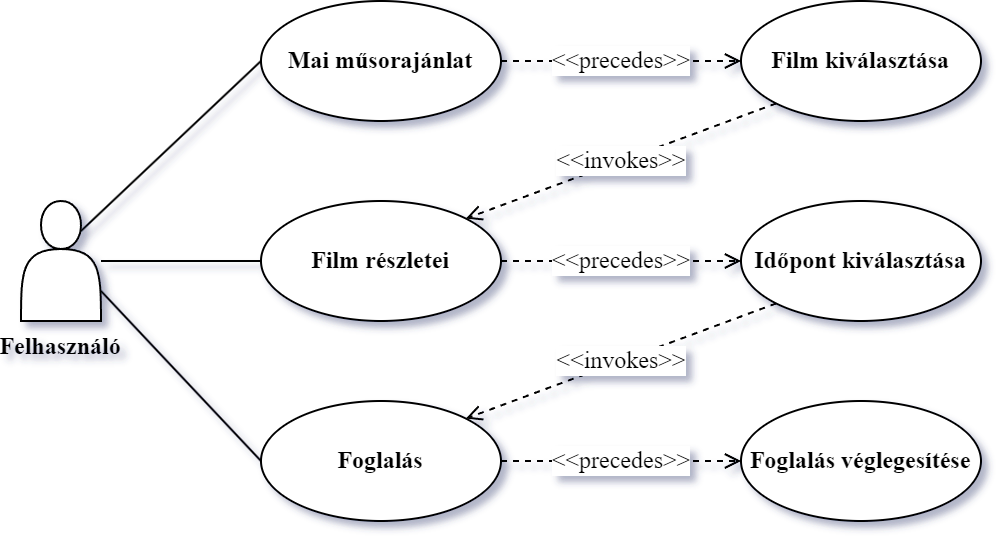
\includegraphics[width=0.75\textwidth]{usercase_web}
		\caption{Webes felület felhasználói eseteinek UML diagramja}
	\end{figure}
	\begin{figure}[H]
		\centering
		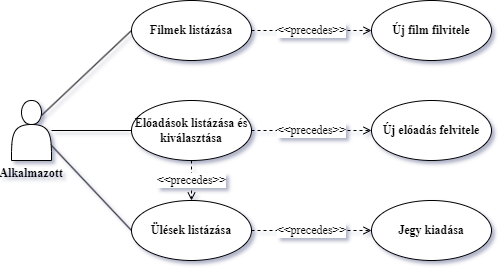
\includegraphics[width=0.75\textwidth]{usercase_desktop}
		\caption{Asztali grafikus felület felhasználói eseteinek UML diagramja}
	\end{figure}
	\subsection*{Rendszer szerkezete}
	\begin{figure}[H]
		\centering
		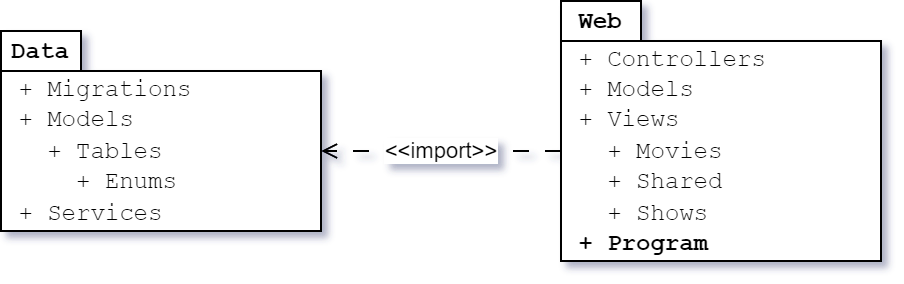
\includegraphics[width=0.75\textwidth]{component}
		\caption{Komponensek UML diagramja}
	\end{figure}
	\begin{itemize}
		\item A rendszer a részeknek megfelelően négy projektből és azok névtereiből épül fel:
		\begin{enumerate}
			\item Az adatbázis modellt (\texttt{Models} és \texttt{Migrations} névterek) és annak adatátviteli osztályait (\texttt{DTOs} névtér) tartalmazó \texttt{Cinema.Data} projekt
			\begin{enumerate}
				\item \texttt{Cinema.Data.Models} névtér az adatbázis sémájának és azok tábláinak definícióit tartalmazza, melynek tartalmát a \texttt{Cinema.Data.Migrations} névtérbe fordítja egy migráció esetén, mellyel futtatáskor áll fel az adatbázis
				\item \texttt{Cinema.Data.DTOs} névtér az adatbázis adatátviteli osztályait tartalmazza, amely előre megírt szűrőkként szolgálnak az asztali grafikus felülethez
			\end{enumerate}
			\begin{figure}[H]
				\centering
				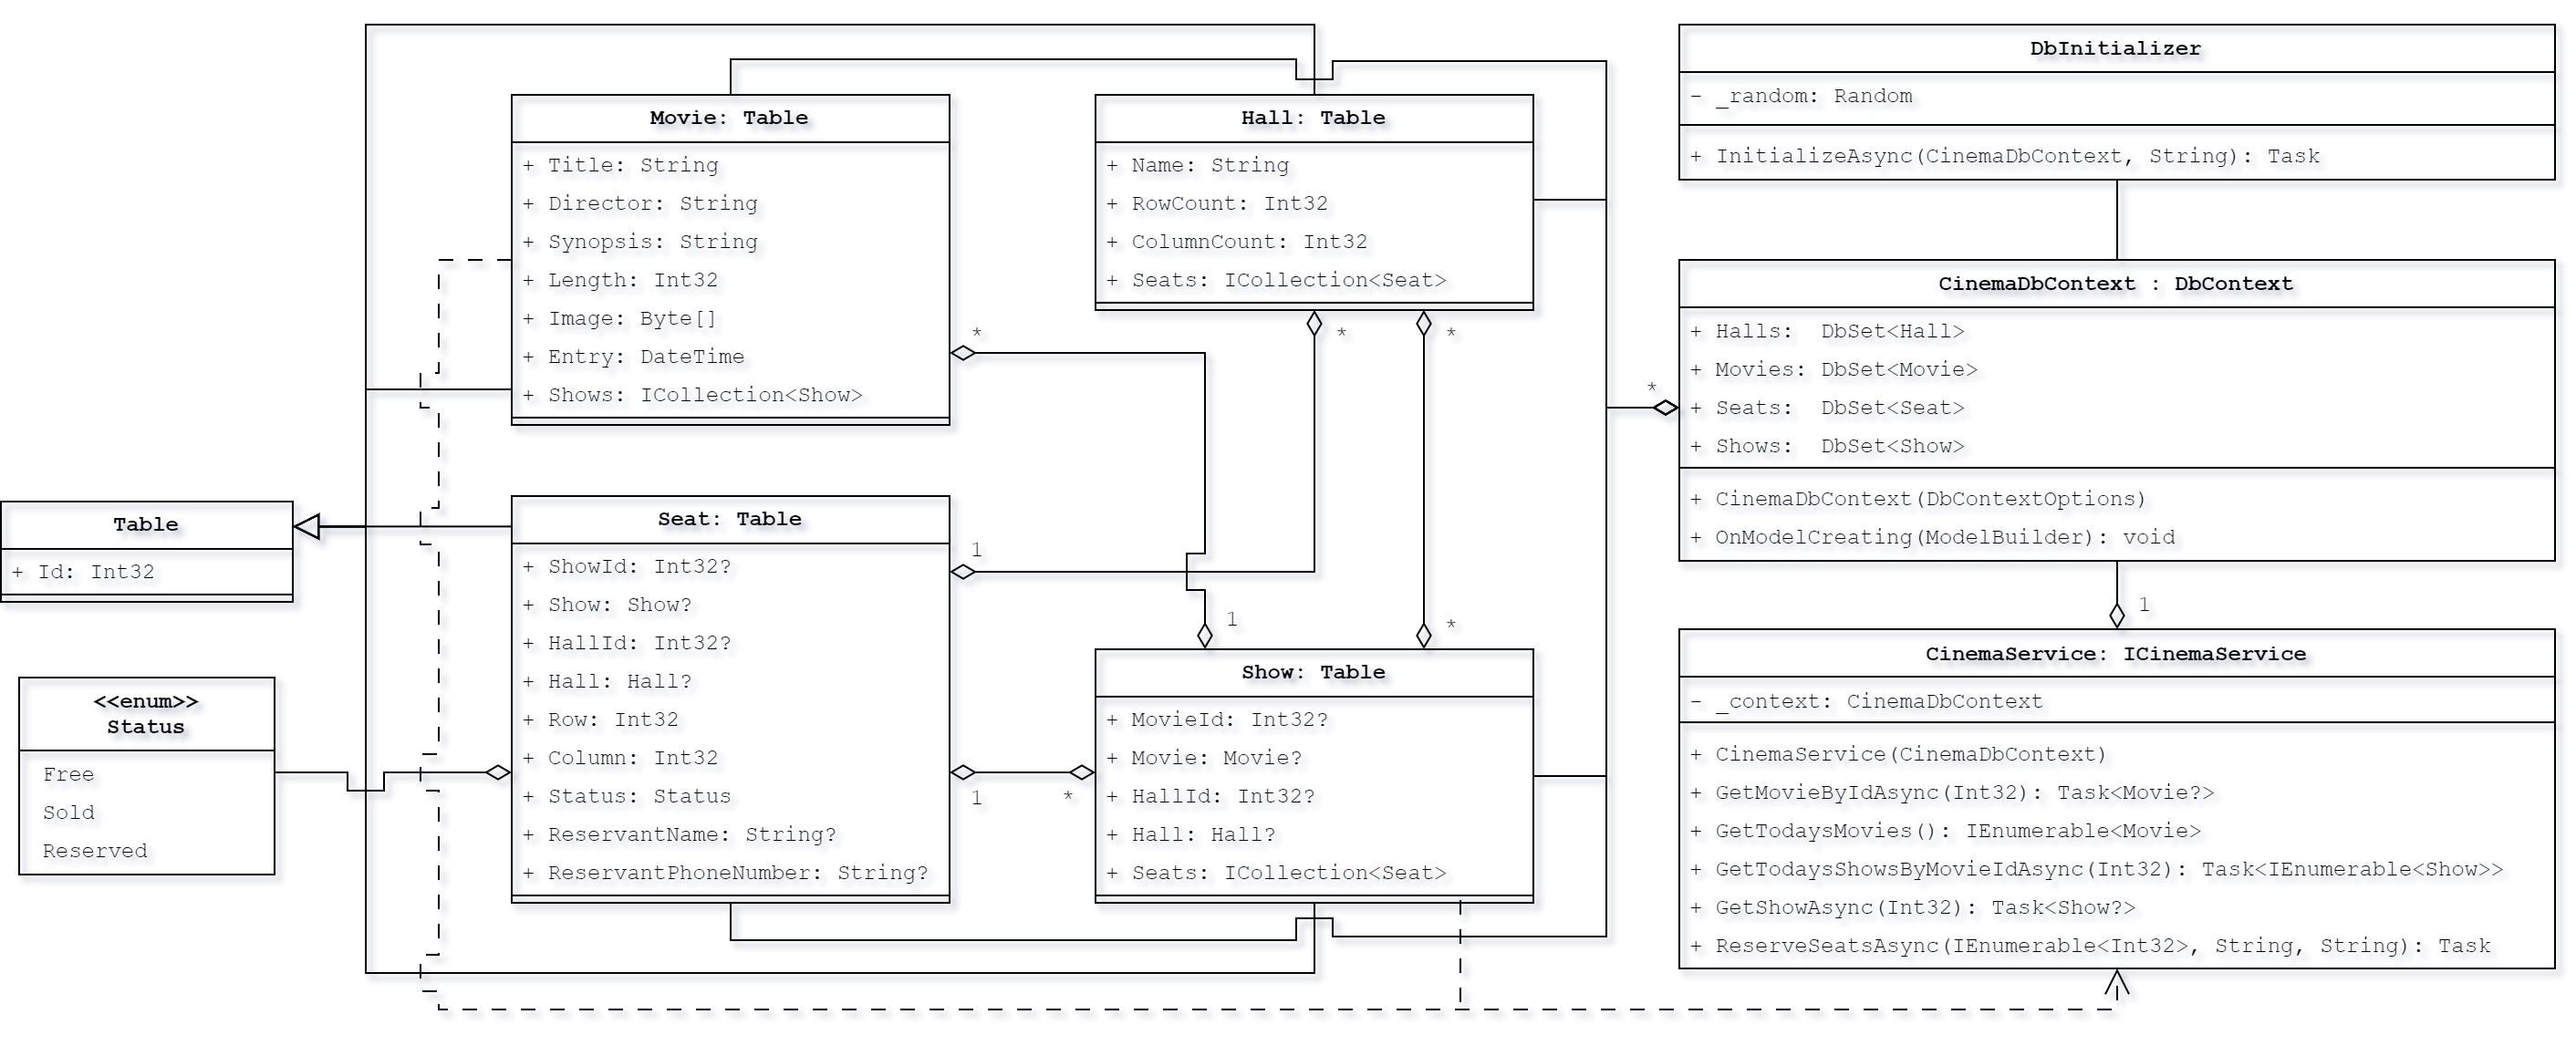
\includegraphics[width=1\textwidth]{data}
				\caption{A \texttt{Cinema.Data} projekt UML osztálydiagramja}
			\end{figure}\newpage
			\item A kontrollerosztályokat (\texttt{Controllers} névtér), az adatátviteli osztályokat (\texttt{Models} névtér) és a webes felhasználói felületet (\texttt{Views} névtér) tartalmazó \texttt{Cinema.Web} projekt
			\begin{enumerate}
				\item \texttt{Cinema.Web.Controllers} névtér az adatbázisból kapott szervízosztály előre megírt lekérdezéseinek az eredményét a \texttt{Cinema.Web.Models} névtérben definiált adatátviteli objektumokká alakítva továbbítja a webes felhasználói felület "dinamikus összeállítójának"
				\item \texttt{Cinema.Web.Views} névtér a webes felhasználói felület weblapjainak a "tervrajzait" tartalmazza \texttt{.cshtml} kiterjesztésben, amely a kapott adatoknak megfelelően szerveroldalon állítja össze a weblapot, majd küldi azt tovább a felhasználónak
			\end{enumerate}
			\begin{figure}[H]
				\centering
				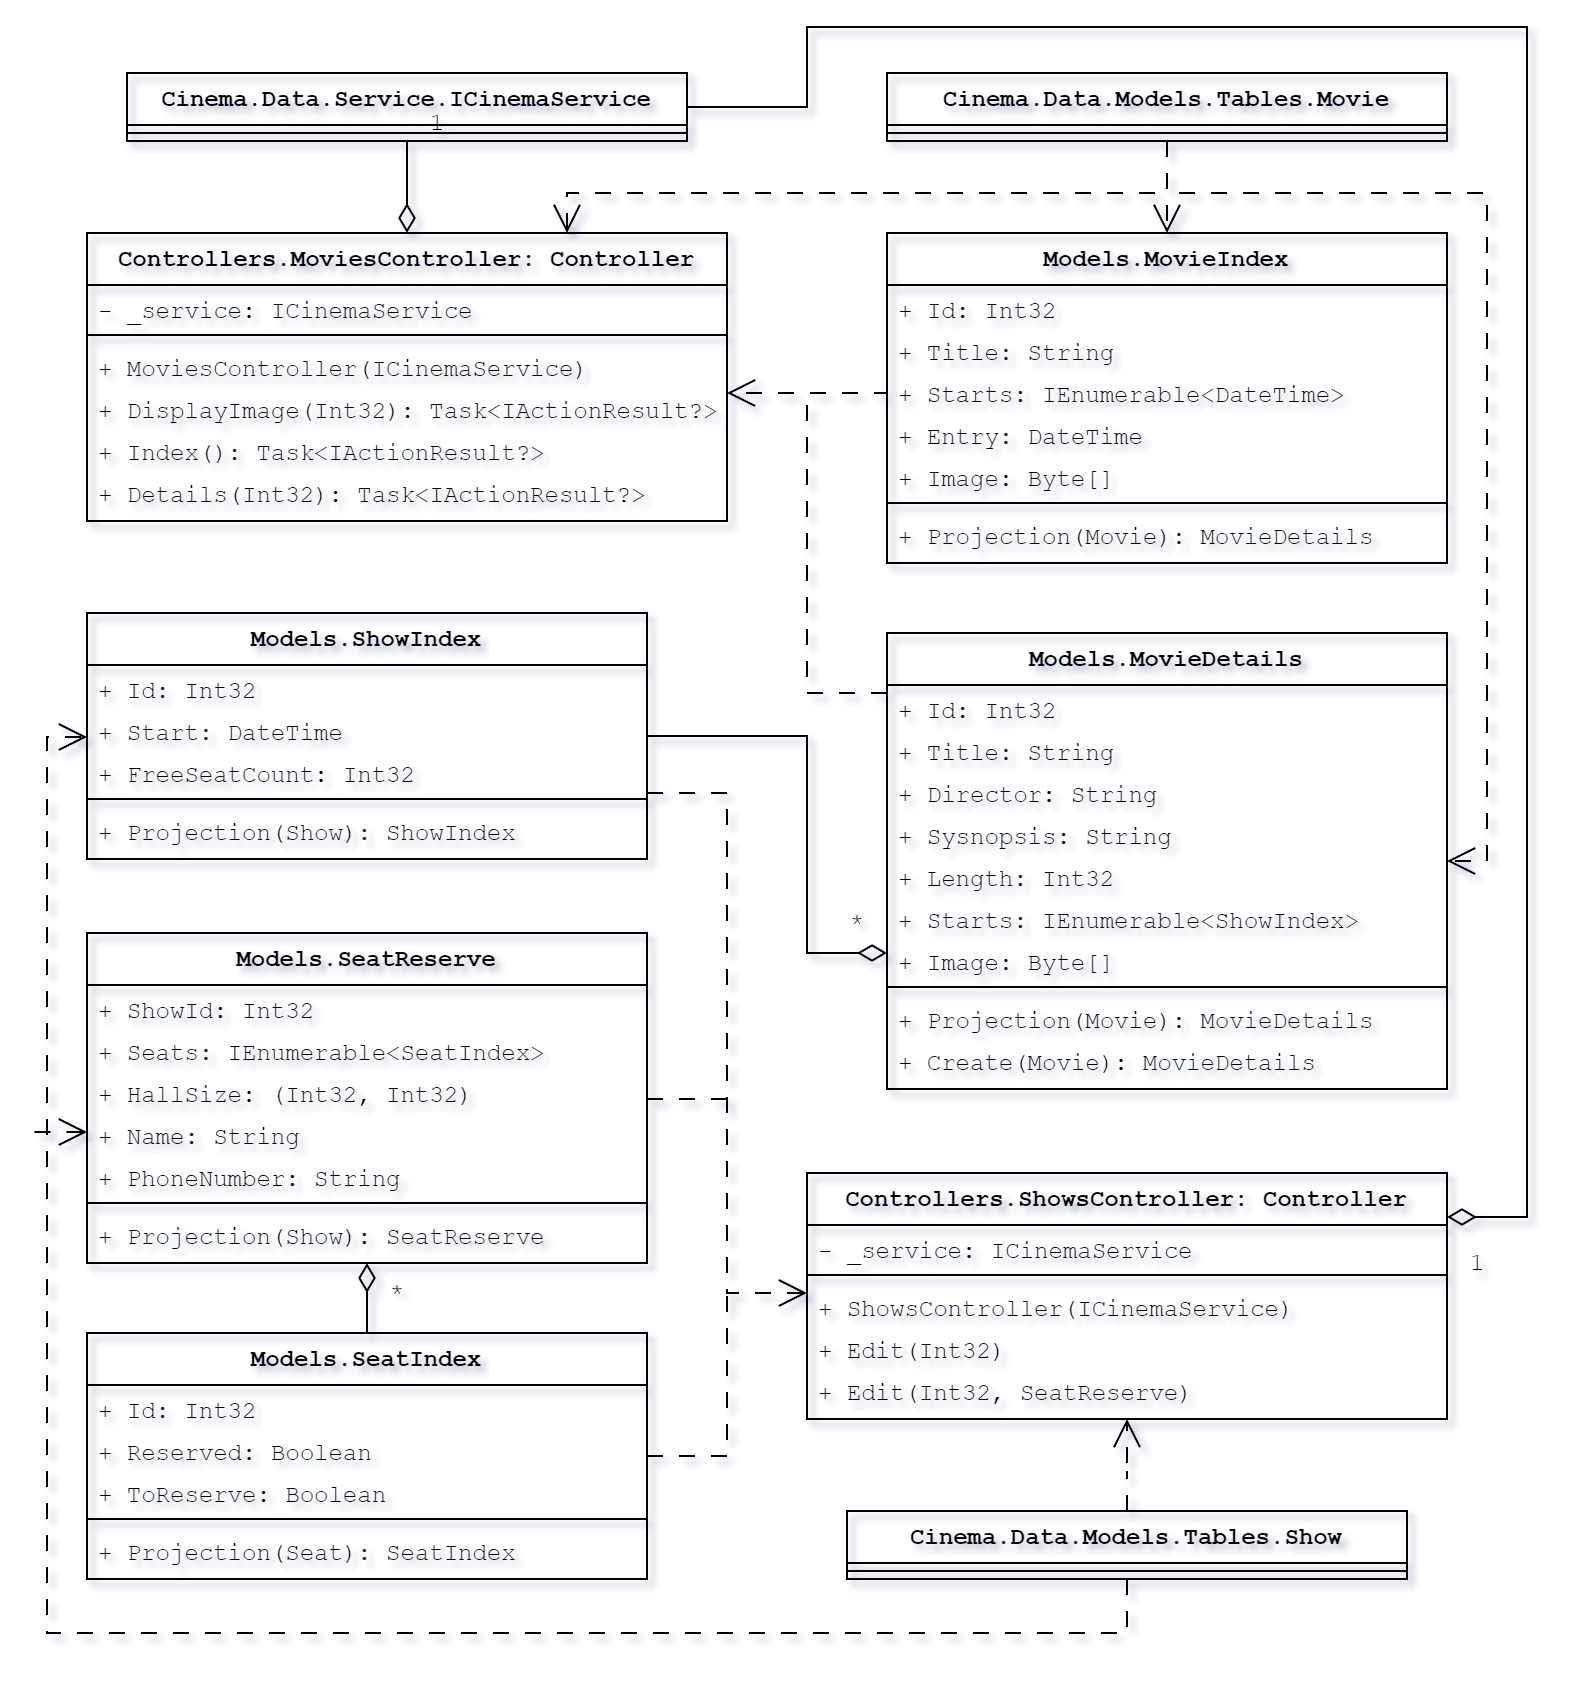
\includegraphics[width=\textwidth]{web}
				\caption{A \texttt{Cinema.Web} projekt UML osztálydiagramja}
			\end{figure}
			\item A webszolgáltatás kontrollerosztályait (\texttt{Cinema.WebAPI.Controllers} névtér) tartalmazó \texttt{Cinema.WebAPI} projekt, mely az asztali grafikus felület számára továbbít adatokat az adatbázisból.
			\begin{figure}[H]
				\centering
				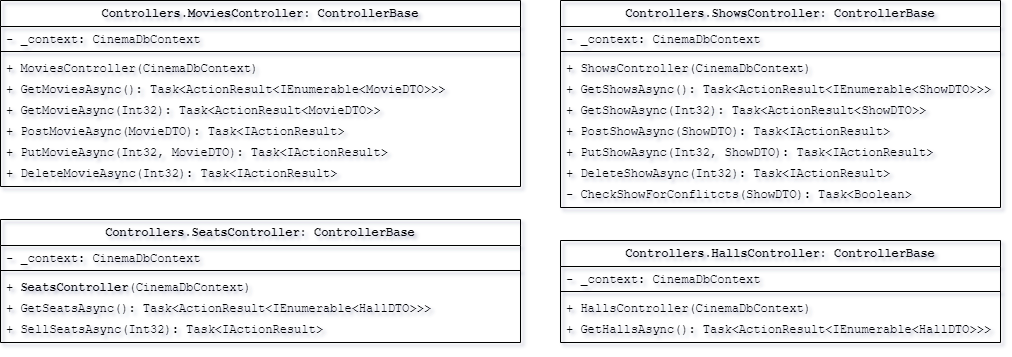
\includegraphics[width=\textwidth]{webapi}
				\caption{A \texttt{Cinema.WebAPI} projekt UML osztálydiagramja}
			\end{figure}
			\item Az asztali grafikus felület modelljét (\texttt{Model} névtér), nézetmodelljét (\texttt{ViewModel} névtér) és nézetét (\texttt{View} névtér) tartalmazó \texttt{Cinema.Admin} projekt
			\begin{enumerate}
				\item \texttt{Cinema.Admin.Model} névtér a webszolgáltatástól megkapott adatokat konvertálja a projekt számára hasznosítható formátumúra
				\item \texttt{Cinema.Admin.ViewModel} névtér definiálja a nézet által használható formátumú adatokat, mely nem csak tárolja azokat, hanem különféle események kezelésével jelzi, ha azok változnak
				\item \texttt{Cinema.Admin.View} névtér definiálja az ablakok és azok oldalainak megjelenését és tartalmainak elrendezését
			\end{enumerate}
				\begin{figure}[H]
				\centering
				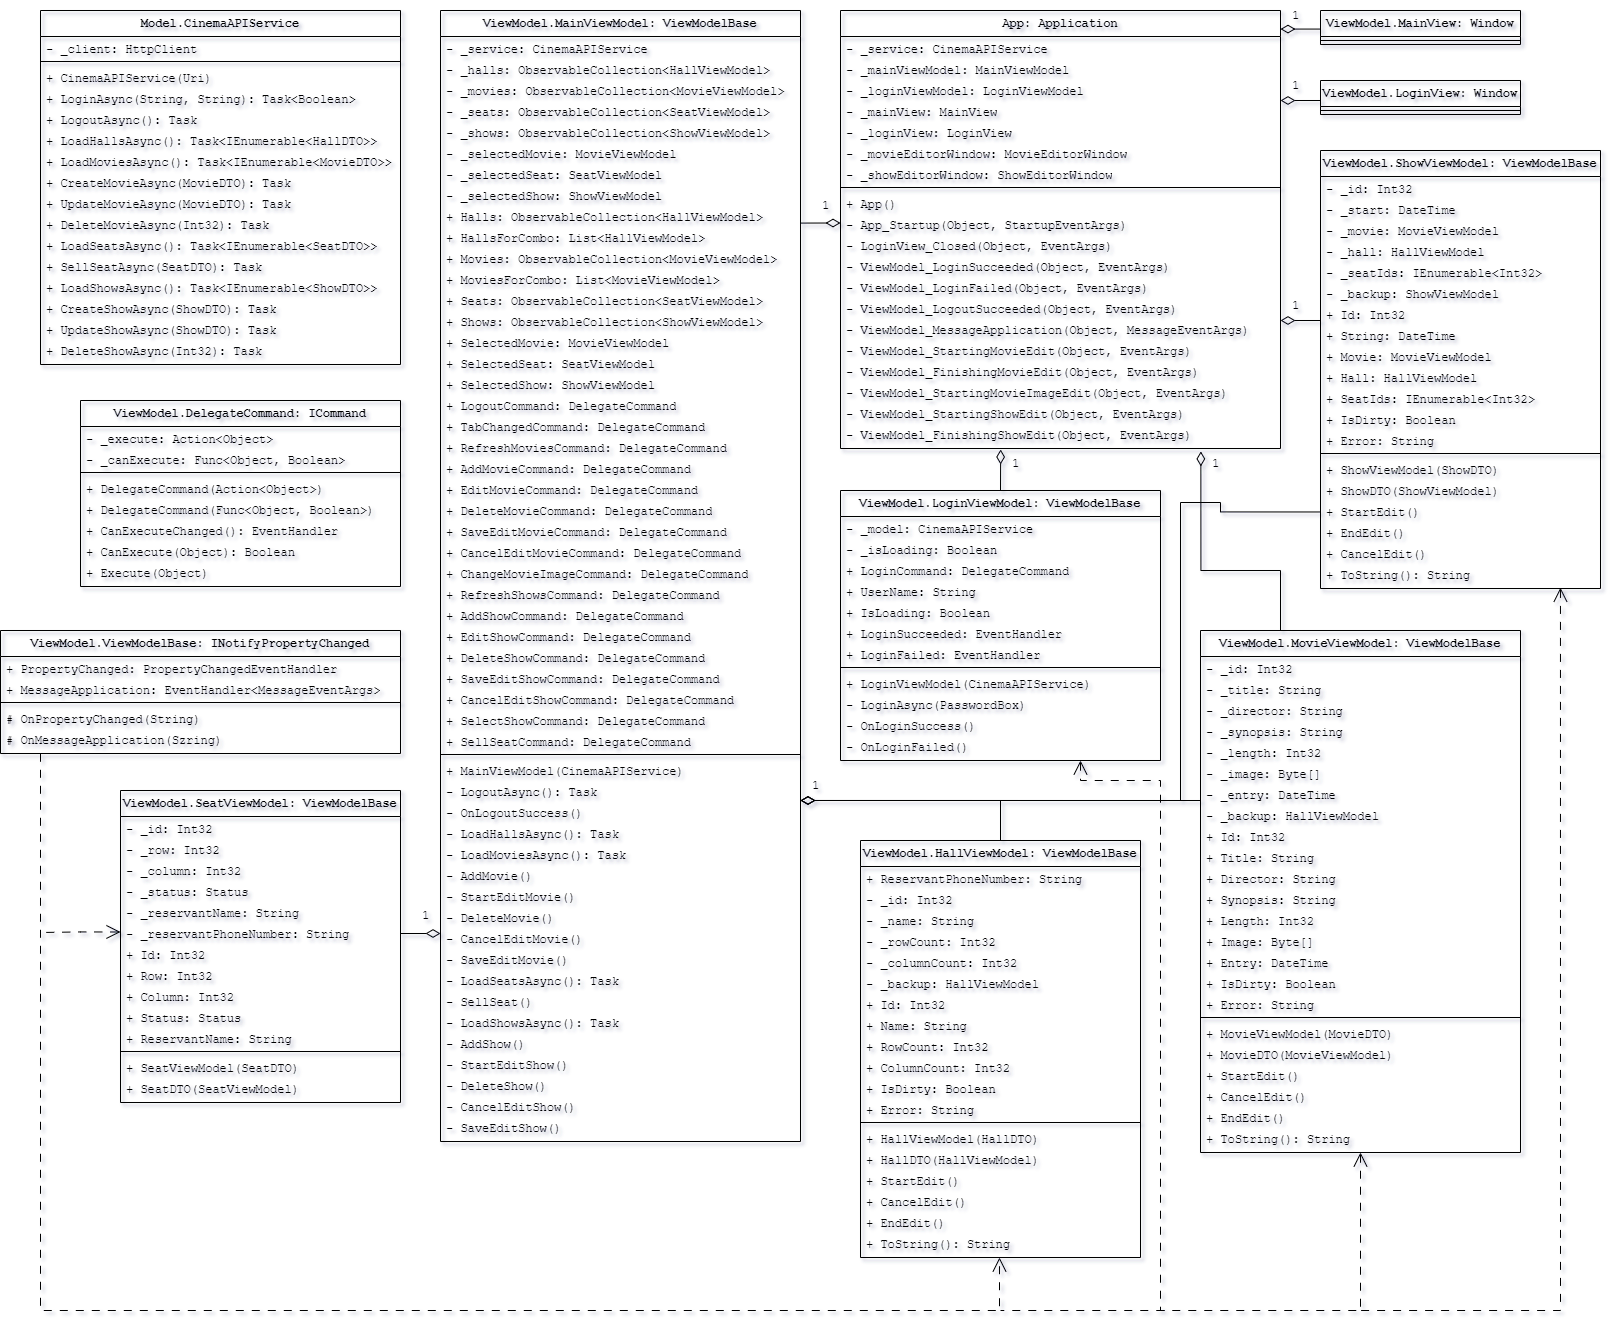
\includegraphics[width=\textwidth]{admin}
				\caption{Az \texttt{Cinema.Admin} modeljének és nézetmodeljének sémájának diagramja}
			\end{figure}
		\end{enumerate}
	\end{itemize}
	\subsection*{Adatbázis felépítése}
	\begin{figure}[H]
		\centering
				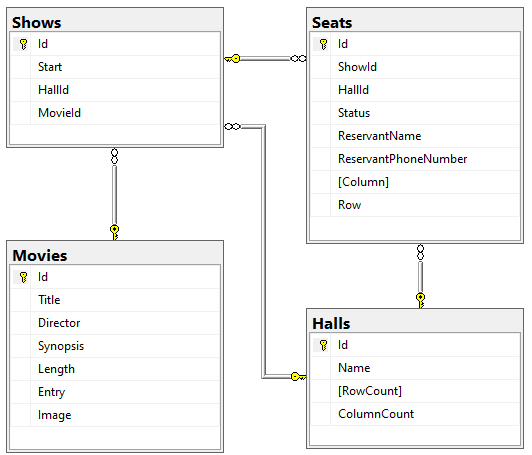
\includegraphics[width=\textwidth]{database}
		\caption{Az adatbázis sémájának diagramja}
	\end{figure}
\end{document}